\section{Electromagnetic calorimeter}
The electromagnetic calorimeter (ECAL) is used to measure the energy deposited by 
electrons, photons, and jets. Due to the high collision rate (collisions happen after 
every 25\unit{ns}), the ECAL has to be very fast and responsive. In view of this, most 
part of ECAL is made of lead tungstate (PbWO$_4$) crystals which are birefringent,
tetragonal, and radiation-hard \cite{PbWO4}. A small part is made of the Pb absorber
(placed in the endcap region, primarily to differentiate events coming from 
$H\rightarrow \gamma\gamma$ and $\pi^0 \rightarrow \gamma\gamma$). A typical PbWO$_4$ 
crystal is shown in Figure~\ref{subfig:cms_ecal_PbWO4}. The volume of a PbWO$_4$ crystal is 
roughly equal to the volume of a coffee cup, and the weight of each crystal is 1.5\unit{kg} (the 
density is 8.3\unit{$\rm g/\rm {cm}^3$}). 
The PbWO$_4$ crystals are grouped in to form modules, and the modules are grouped to form 
super-modules. These super-modules are placed in barrel and endcap region of the ECAL as 
shown in Figure~\ref{subfig:cms_ecal_pos}. The ECAL is made up of 76,000 lead tungstate 
crystals (61,200 in the barrel and 14,800 in the endcap region).
%Fig\pdfcomment[author={FIG COURTESY}]{Ecal-pic: https://inspirehep.net/record/1251416/plots, crystal-pic:http://cms.web.cern.ch/news/electromagnetic-calorimeter}}
\begin{figure}
  \centering
	\subfigure[PbWO$_4$ crystal \cite{Collaboration_2008_CMS}
	 \label{subfig:cms_ecal_PbWO4}]
	 {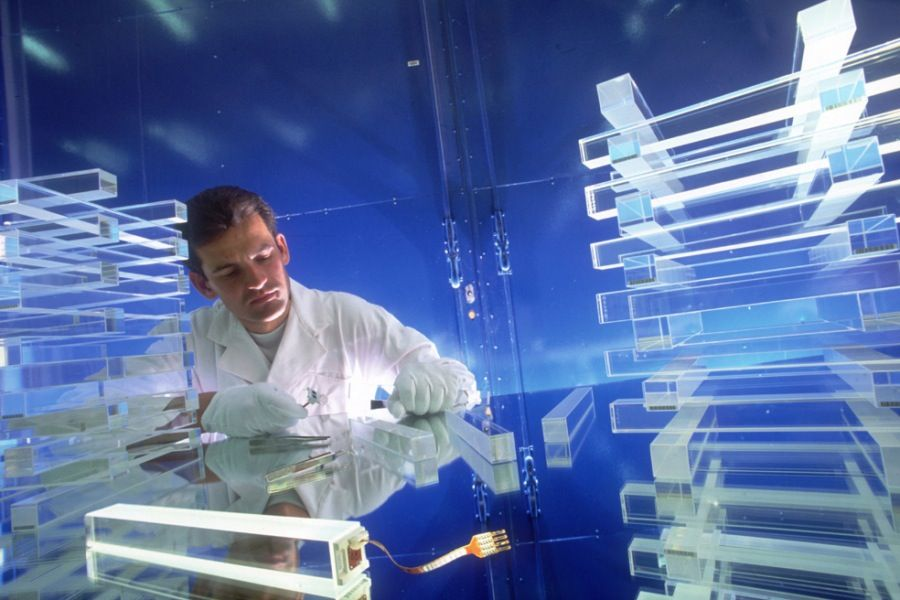
\includegraphics[width=0.40\linewidth]{Experiment/CMS/Image/ECAL/ecal2.jpg}}
	 \hfil
	\subfigure[Components of the ECAL \cite{Collaboration_2008_CMS}
 	\label{subfig:cms_ecal_pos}]
 	{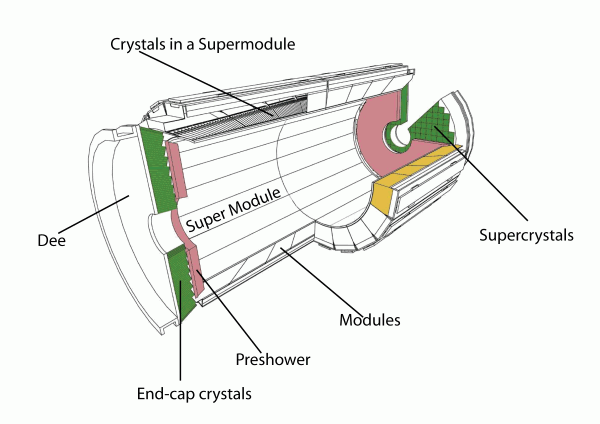
\includegraphics[width=0.40\linewidth]{Experiment/CMS/Image/ECAL/ecal.png}}
 	\caption{(a) A PbWO$_4$ scintillating crystal. (b) The various components of the 
	electromagnetic calorimeter in the barrel and endcap regions.}
 	\label{fig:cms_ecal}
\end{figure}

When a particle passes through the PbWO$_4$ crystals, photons are produced by the
scintillating process. The PbWO$_4$ are inorganic scintillator doped with impurities.
Other inorganic scintillators are alkali halide (NaI+TI, CsI+Na), 
Cerium-activated fast inorganics (LaBr$_3$), etc. Pure crystals such as NaI (octahedral) 
don't produce visible photons so impurities such as TI (activators) are added which 
create special sites in the lattice as shown in Figure~\ref{fig:cms_sinti}. When a
particle passes through the crystal it creates electron-hole pairs. The electrons are 
excited to the conduction band whereas the holes ionise the impurity atoms. The excited 
electron recombines the ionised impurity atoms creating its own excited configurations.
The impurity excited configuration de-excites to the ground state by emitting photons. 
\begin{figure}
  \centering
  {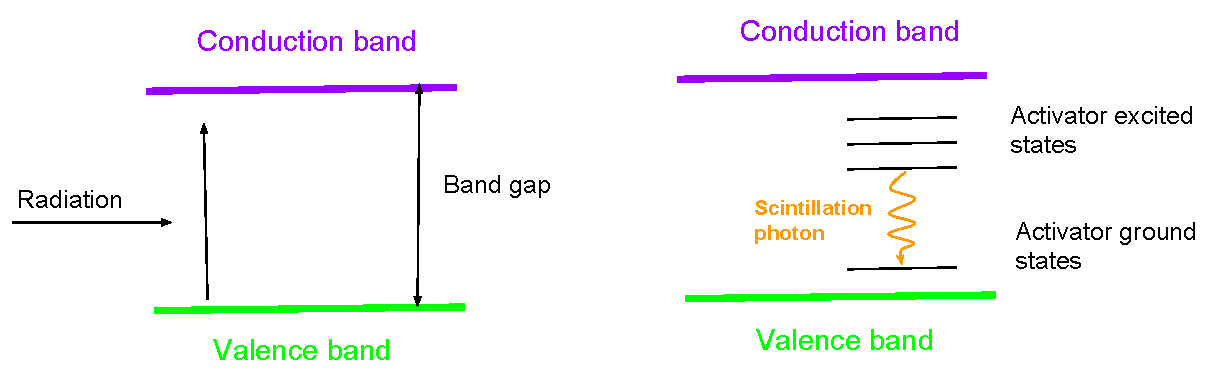
\includegraphics[width=1.0\linewidth]{Experiment/CMS/Image/ECAL/Scintillation.pdf}}
	\caption{The energy band structure in pure (impure) inorganic scintillator shown
	on left (right) side. The impurity creates intermediate excited states between
	the valence and conduction band. The photons are emitted when activator 
	de-excites.}
  \label{fig:cms_sinti}
\end{figure}

The photons thus produced are converted into an electrical signal by the 
photomultiplier tubes (PMTs) or avalanche photodiodes (APDs). The APDs in the
barrel and vacuum phototriodes (VPTs) are placed in the endcap region. The 
electrical signals are amplified and stored. The working principle of PMT is shown 
in Figure~\ref{subfig:cms_pmt}. The photons 
are absorbed on photocathodes. Due to the photoelectric effect, electrons are emitted, 
if the energy of incoming photons is more than $\approx$ 3\unit{eV}. The emitted electrons 
are directed towards the dynodes by an electric field. From the dynodes, the
secondary electrons are emitted with an efficiency (the ratio of number of secondary 
and primary electrons) of $\approx$ 6-8. These electrons are then directed towards 
other dynodes and the process continues. In the end, there are many electrons. 
A schematic diagram of APD is shown in Figure~\ref{subfig:sinti_apd}. When a photon enters 
the depletion region, electron-hole pairs are created. The created electron-holes start moving towards
the respective electrode due to large reverse bias voltage. While moving, they
create additional electron-hole pairs. The process continues producing an avalanche
multiplication.
\begin{figure}
  \centering
	\subfigure[Schematic diagram of photomultiplier tube \cite{pmt}
	 \label{subfig:cms_pmt}]
	 {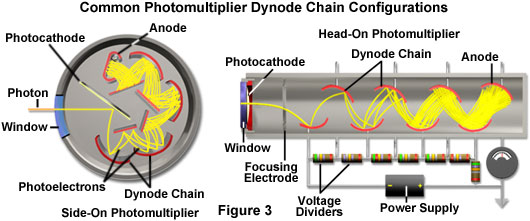
\includegraphics[width=0.50\linewidth]{Experiment/CMS/Image/ECAL/pmt.jpg}}
	 \hfil
	\subfigure[Principle of operation of the avalanche photo-diode \cite{apd}
	 \label{subfig:sinti_apd}]
	 {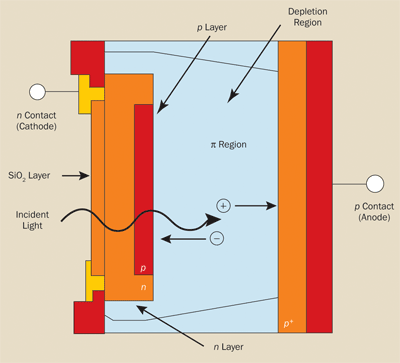
\includegraphics[width=0.30\linewidth]{Experiment/CMS/Image/ECAL/apd.png}}
	 \caption{The schematic diagram of a circular and cylindrical PMT (a). 
	 The principle of operation of an APD is shown in (b).}
	 \label{fig:cms_pmt_apd}
\end{figure}

An electromagnetic pre-shower, as shown in Figure~\ref{subfig:cms_ecal_preS} is placed
in the endcap region at $z$ = 298.5\unit{cm} to distinguish photons coming from Higgs and pion.
The photons produced by the pion ($\pi^0$) are likely to be narrowly separated and
will be traveling in the forward direction. However, those coming from the Higgs 
are well separated and mostly in the transverse direction. Therefore, if
there is a photon in an event which was reconstructed using the preshower then
it most likely came from the $\pi$ decay and can be rejected for the study of
$H \rightarrow \gamma \gamma$ process.
The preshower has a diameter of 240\unit{cm} with a thickness of 20\unit{cm}. It 
has alternate layers of absorber and detectors on both sides of its center. 
Electromagnetic showers are produced from lead layers when a photon passes through it, 
which silicon sensors detect. The two layers are used to determine the position of the 
particles. 
\begin{figure}
  \centering
	\subfigure[Preshower disk 
  \label{subfig:cms_ecal_preS}]
  {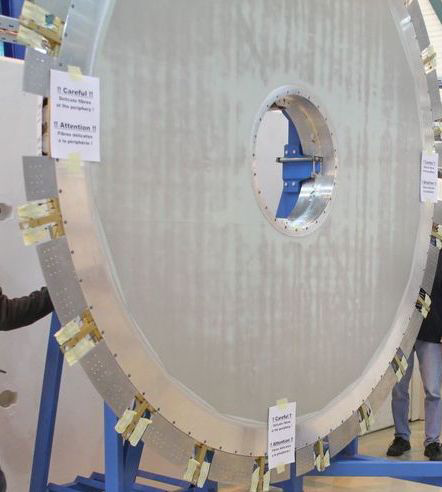
\includegraphics[width=0.30\linewidth]{Experiment/CMS/Image/ECAL/ecal3.png}}
  \hfil
  \subfigure[Composition of preshower
  \label{subfig:sinti_ecal_preS_pos}]
  {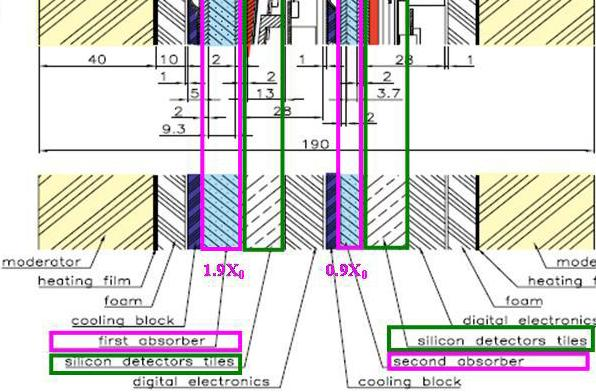
\includegraphics[width=0.50\linewidth]{Experiment/CMS/Image/ECAL/ecal4.jpg}}
  \caption{ECAL preshower \cite{preS} placed in the endcap region at $z$ = 298.5\unit{cm}. The 
	preshower is made of alternate layers starting from the moderator, to 
	heating film to foam to cooling block to the absorber (Pb) to silicon
	detectors to the digital electronics. The width of the lead (Pb) absorber
	is not the same on both sides.}
  \label{fig:cms_ecal_pre}
\end{figure}

For a given energy \textit{E} (in \GeV), the energy resolution of ECAL is given by 
\cite{Chatrchyan:2013dga}
\begin{equation}
	\frac{\sigma_E}{E} = \frac{2.8\%}{\sqrt{E}} \oplus \frac{12.8\%}{E} \oplus 0.3\%
	\label{eq:cms_ecal_reso}
\end{equation}
where the terms in the quadrature sum correspond to the stochastic correction which accounts
for the energy deposited in the preshower and event-by-event fluctuations, the noise term
due to noise in backend electronics, and a constant term which takes into account
the non-uniformity of the detector and temperature gradient. From 
Equation (\ref{eq:cms_ecal_reso}), it is clear that the stochastic and noise term 
dominate at lower energies whereas the constant term becomes dominant at higher energies. 

The relative energy resolution as a function of $\eta$ of supercluster 
($ 3\times 3$ crystal) for electron and photon is shown in 
Figure~\ref{fig:cms_ecal_reso}. The relative resolution is shown in both barrel and
endcap region for $R_9 < 0.94$, $R_9 > 0.94$, where $R_9$ is a cluster shape parameter 
defined as $\rm{max}(E_{3\times 3})/E_{\rm{sc}}$. The $\rm{max}(E_{3\times 3})$ is the 
maximum energy deposited in a particular crystal out of 9 crystal, and $E_{\rm{sc}}$ is
the energy deposited in the supercluster, that is, the sum of energy deposited in all 9
crystals \cite{Chatrchyan:2013dga}. The relative energy resolution from observed data,
simulated MC, and smeared MC were determined 
at $\sqrt{s} = 7$ \TeV. The relative resolutions are better in the barrel as compared to 
the endcap region for $R_9 < 0.94$ as well as $R_9 > 0.94$ for electron and photon. From data, 
the minimum (maximum) resolution is about 1\% (5\%) for both electron and photon.

\begin{figure}
  \centering
  \subfigure[]
  {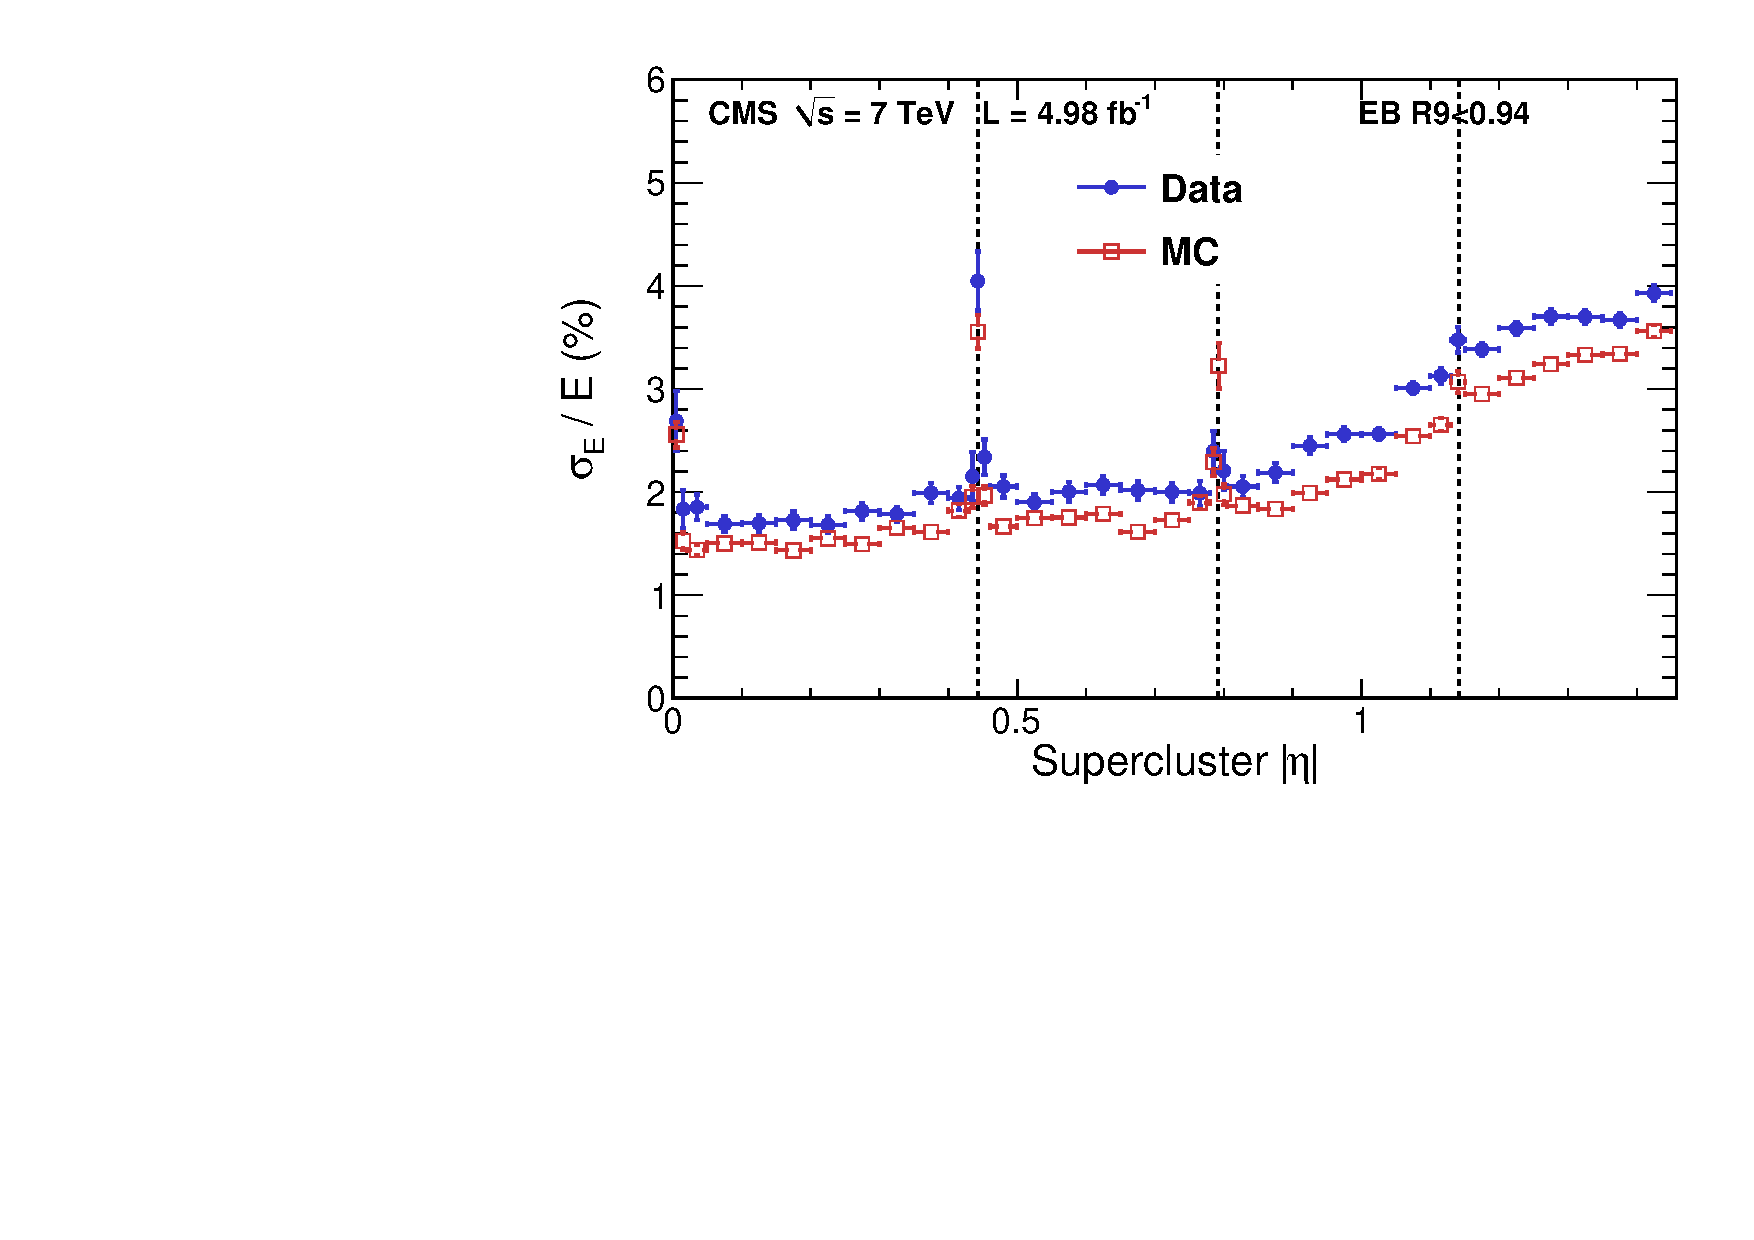
\includegraphics[width=0.39\linewidth]{Experiment/CMS/Image/ECAL/SCe_EtaR9calib_regression_EB_ER_ir9_0.pdf}}
  \subfigure[]
  {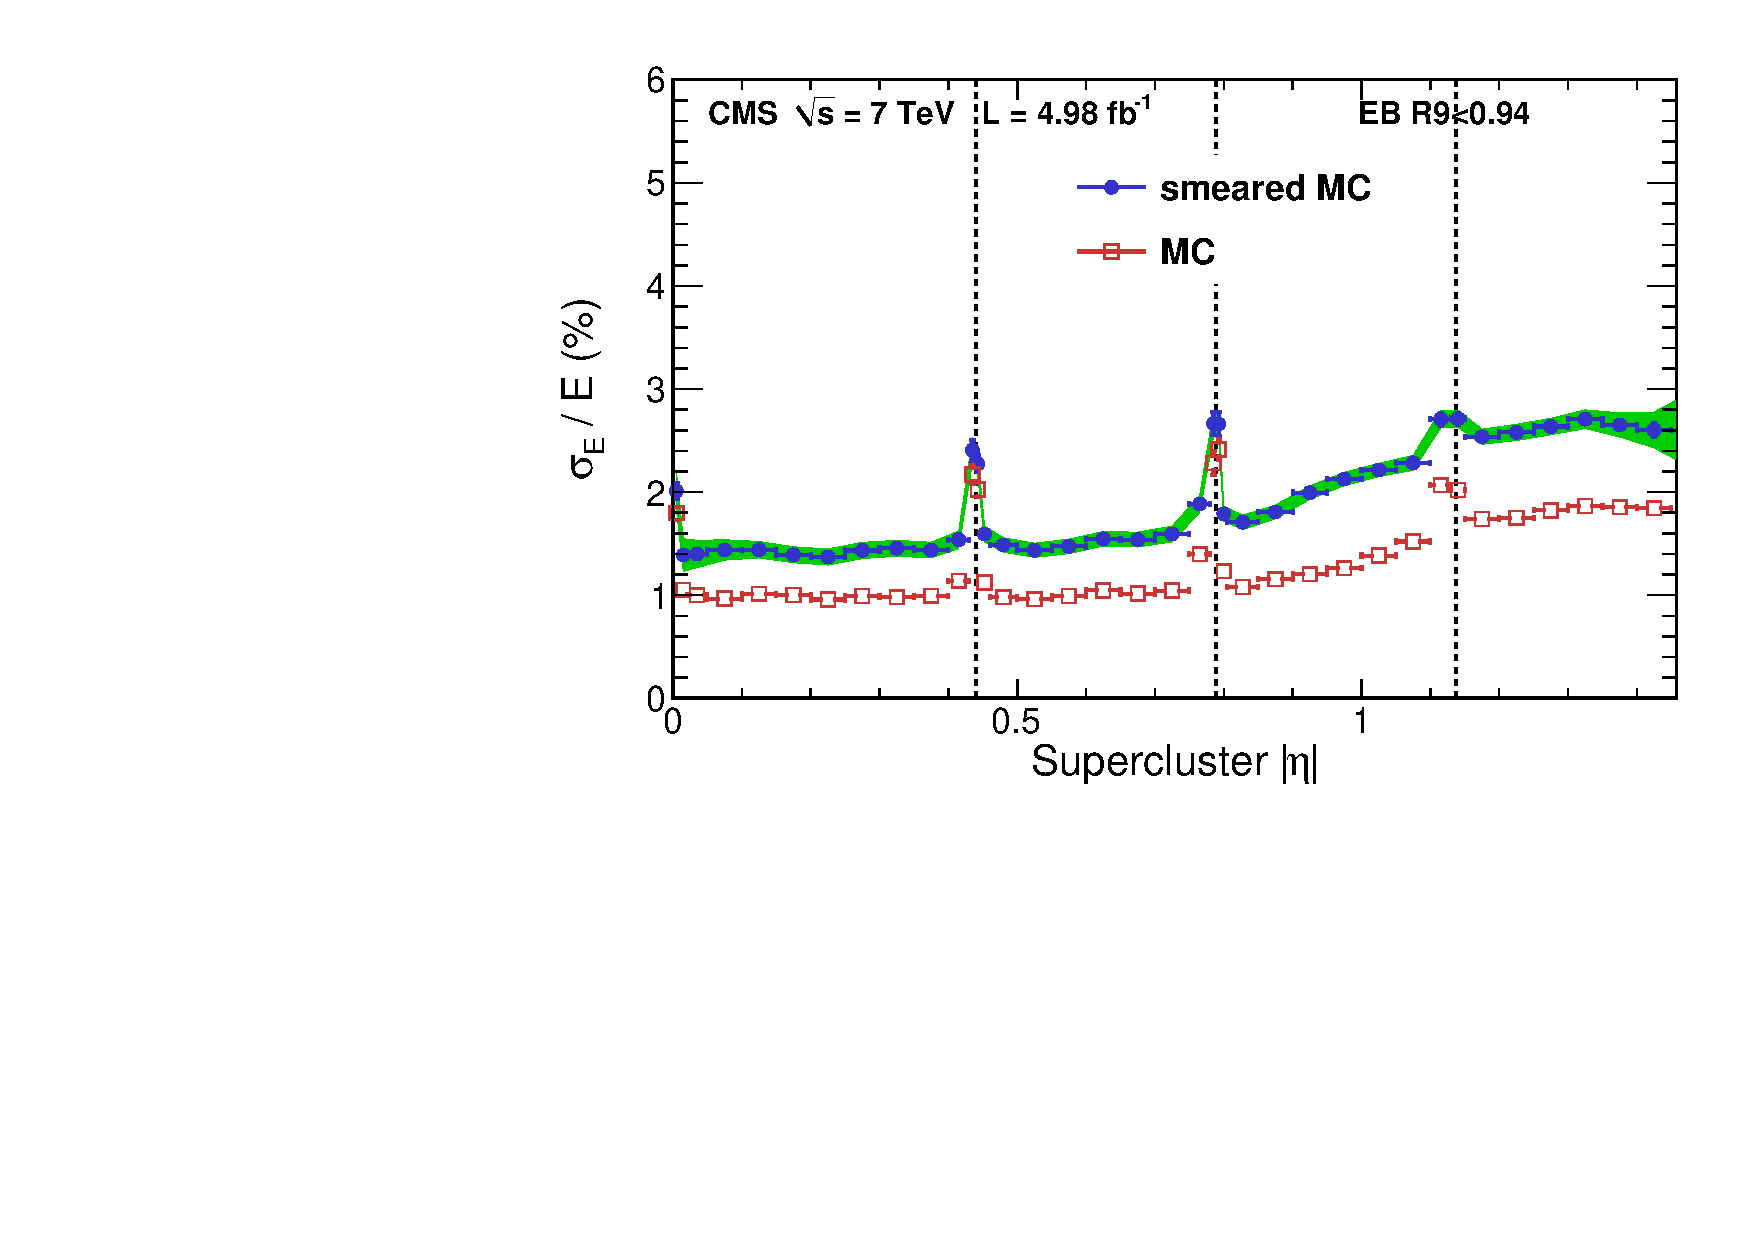
\includegraphics[width=0.39\linewidth]{Experiment/CMS/Image/ECAL/SCphoton_Reso_EB_ER_ir9_0.pdf}}
  \vfil
  \subfigure[]
  {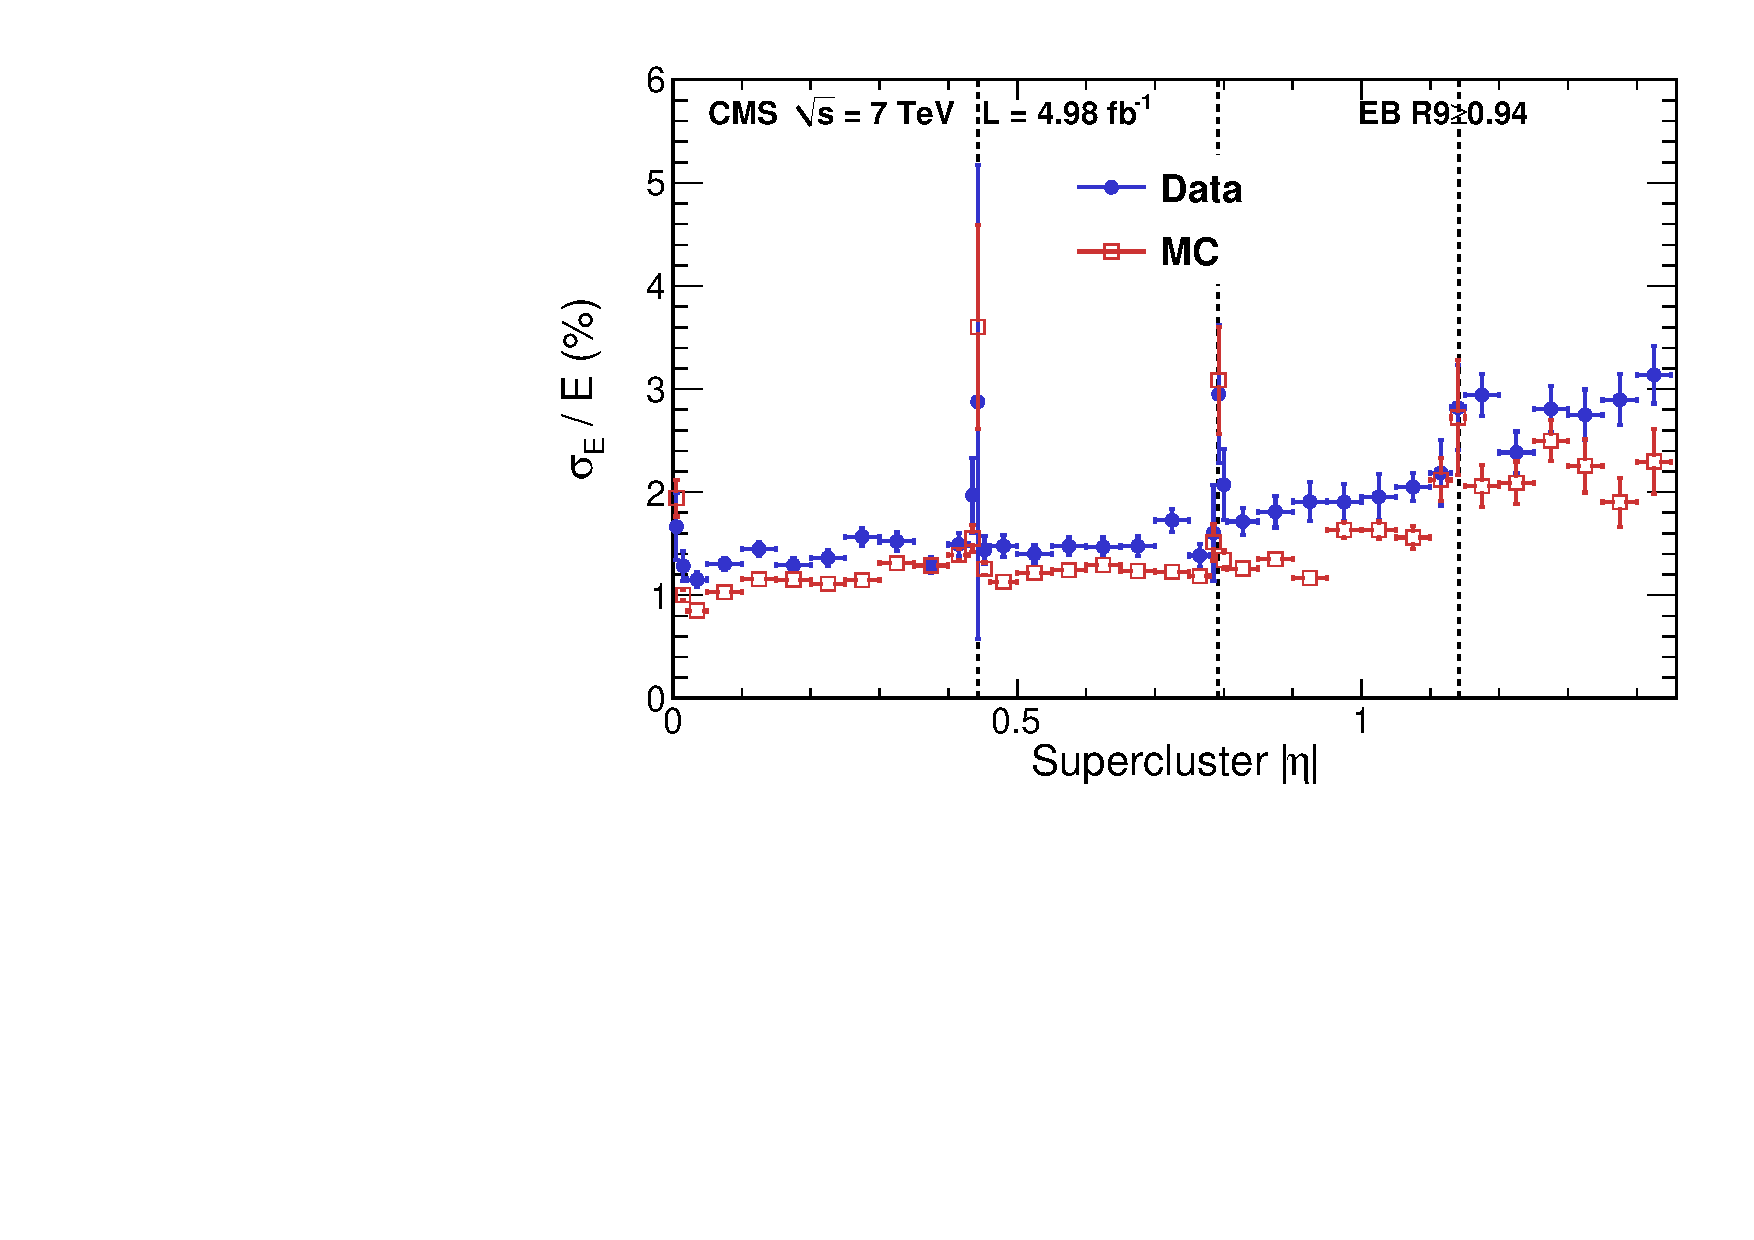
\includegraphics[width=0.39\linewidth]{Experiment/CMS/Image/ECAL/SCe_EtaR9calib_regression_EB_ER_ir9_1.pdf}}
  \subfigure[]
  {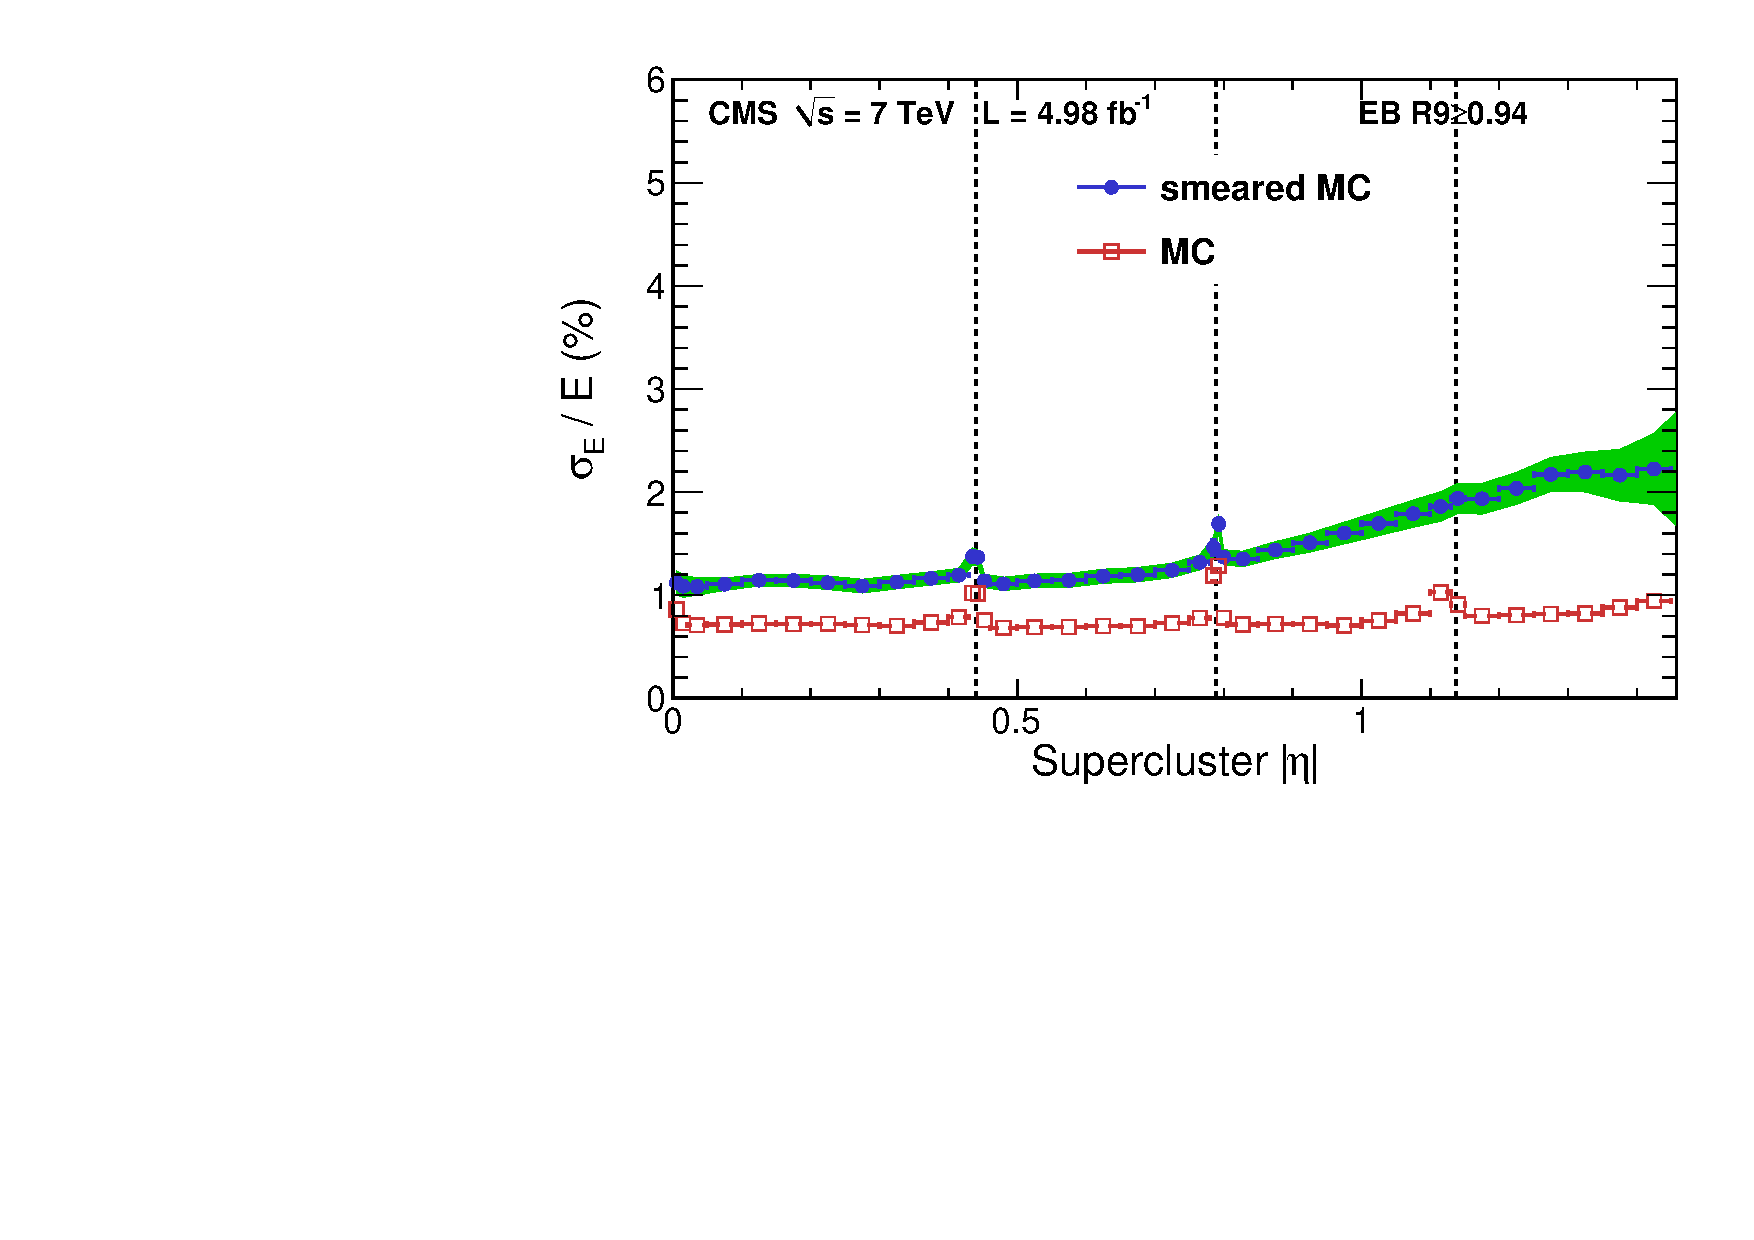
\includegraphics[width=0.39\linewidth]{Experiment/CMS/Image/ECAL/SCphoton_Reso_EB_ER_ir9_1.pdf}}
  \vfil
  \subfigure[]
  {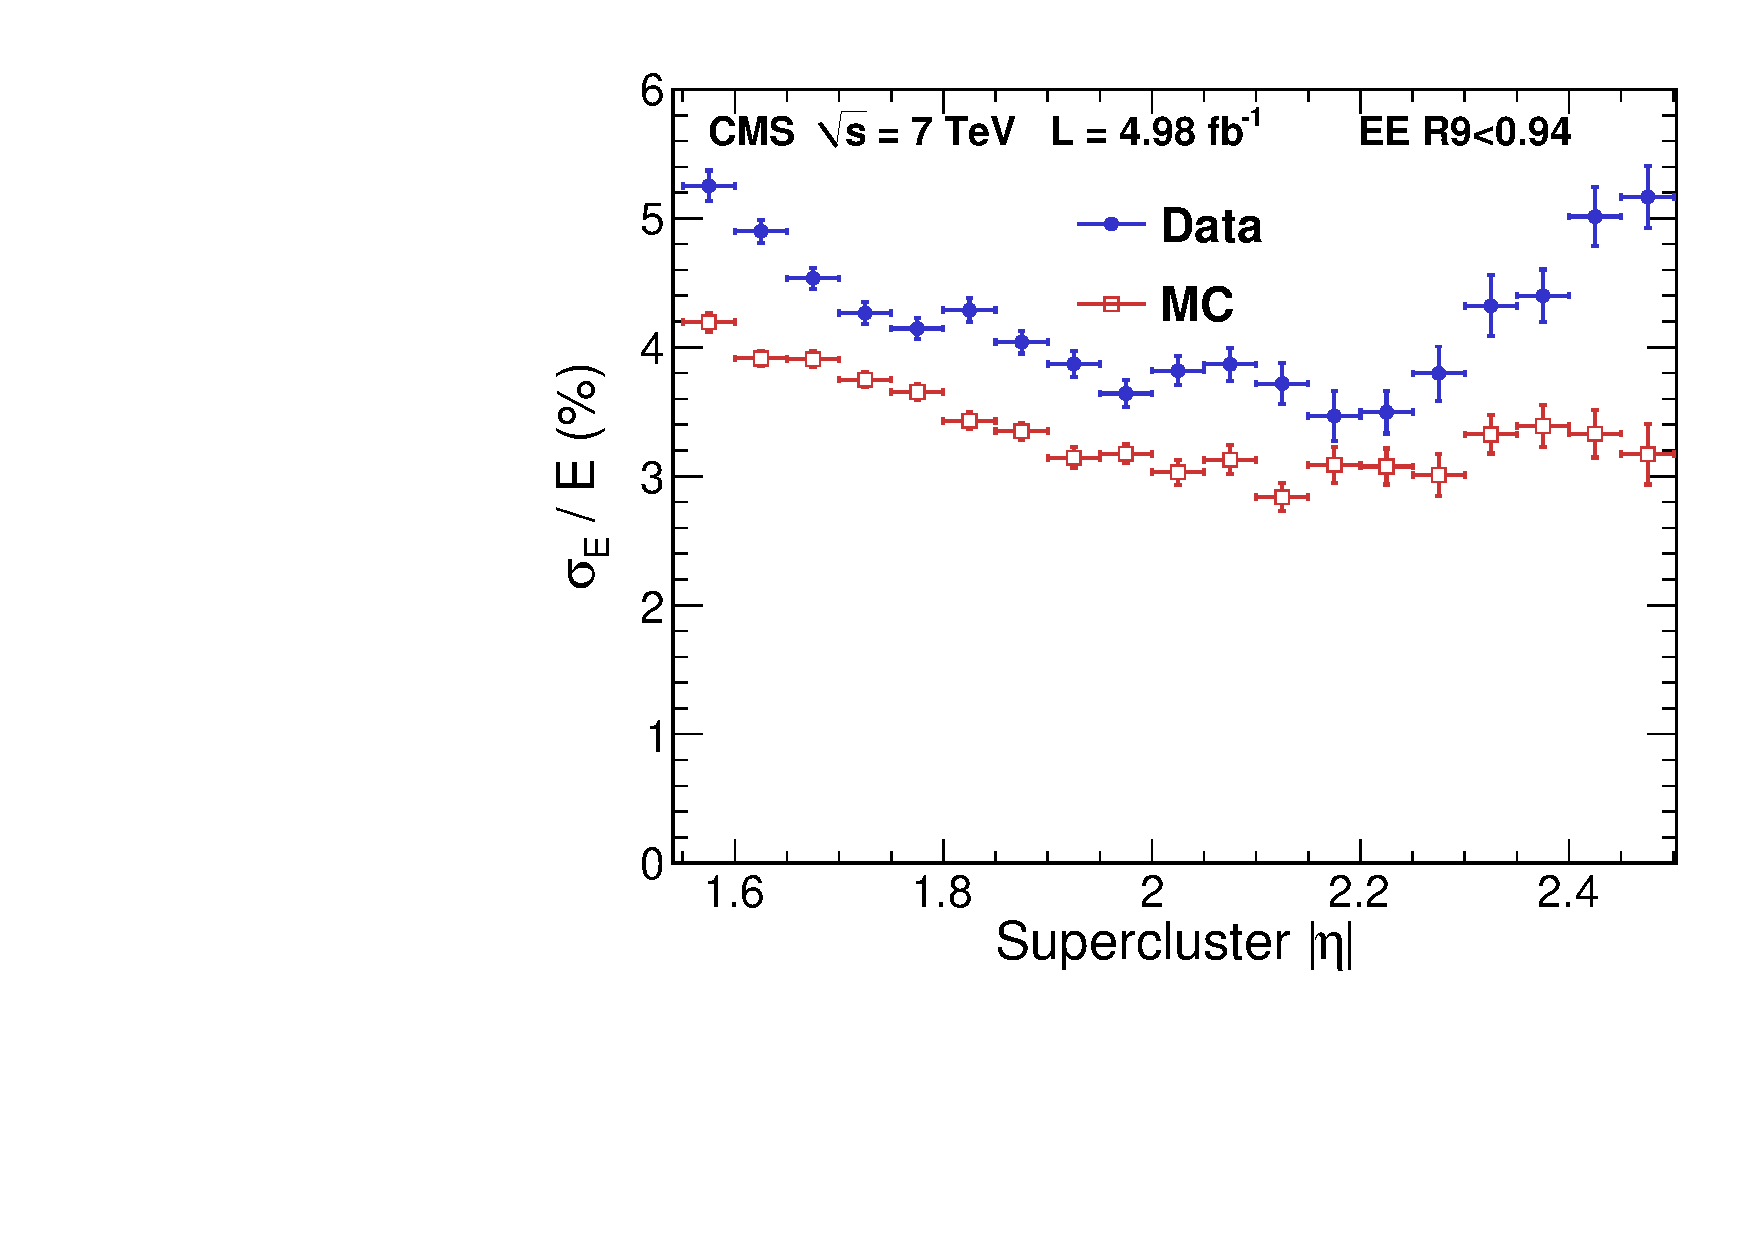
\includegraphics[width=0.39\linewidth]{Experiment/CMS/Image/ECAL/SCe_EtaR9calib_regression_EE_ER_ir9_0.pdf}}
  \subfigure[]
  {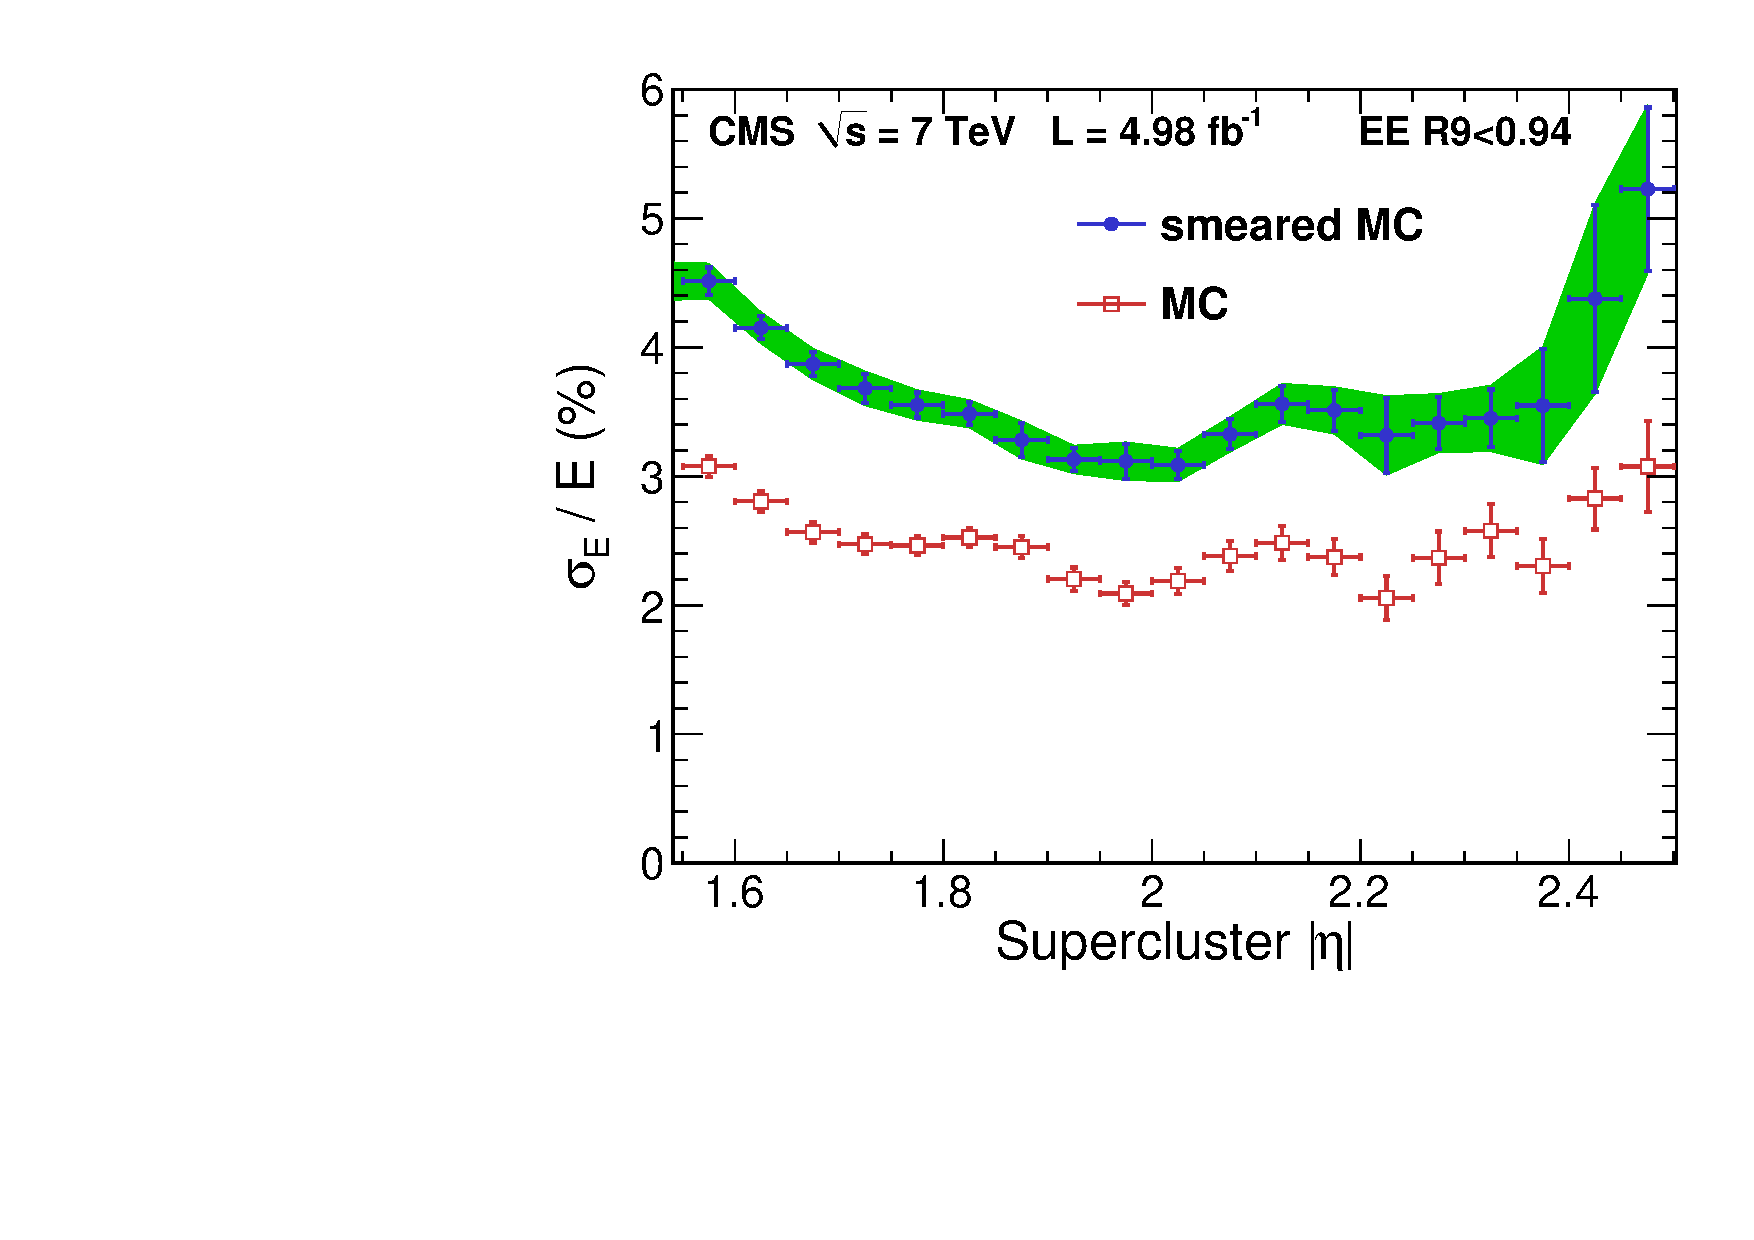
\includegraphics[width=0.39\linewidth]{Experiment/CMS/Image/ECAL/SCphoton_Reso_EE_ER_ir9_0.pdf}}
  \vfil
  \subfigure[]
  {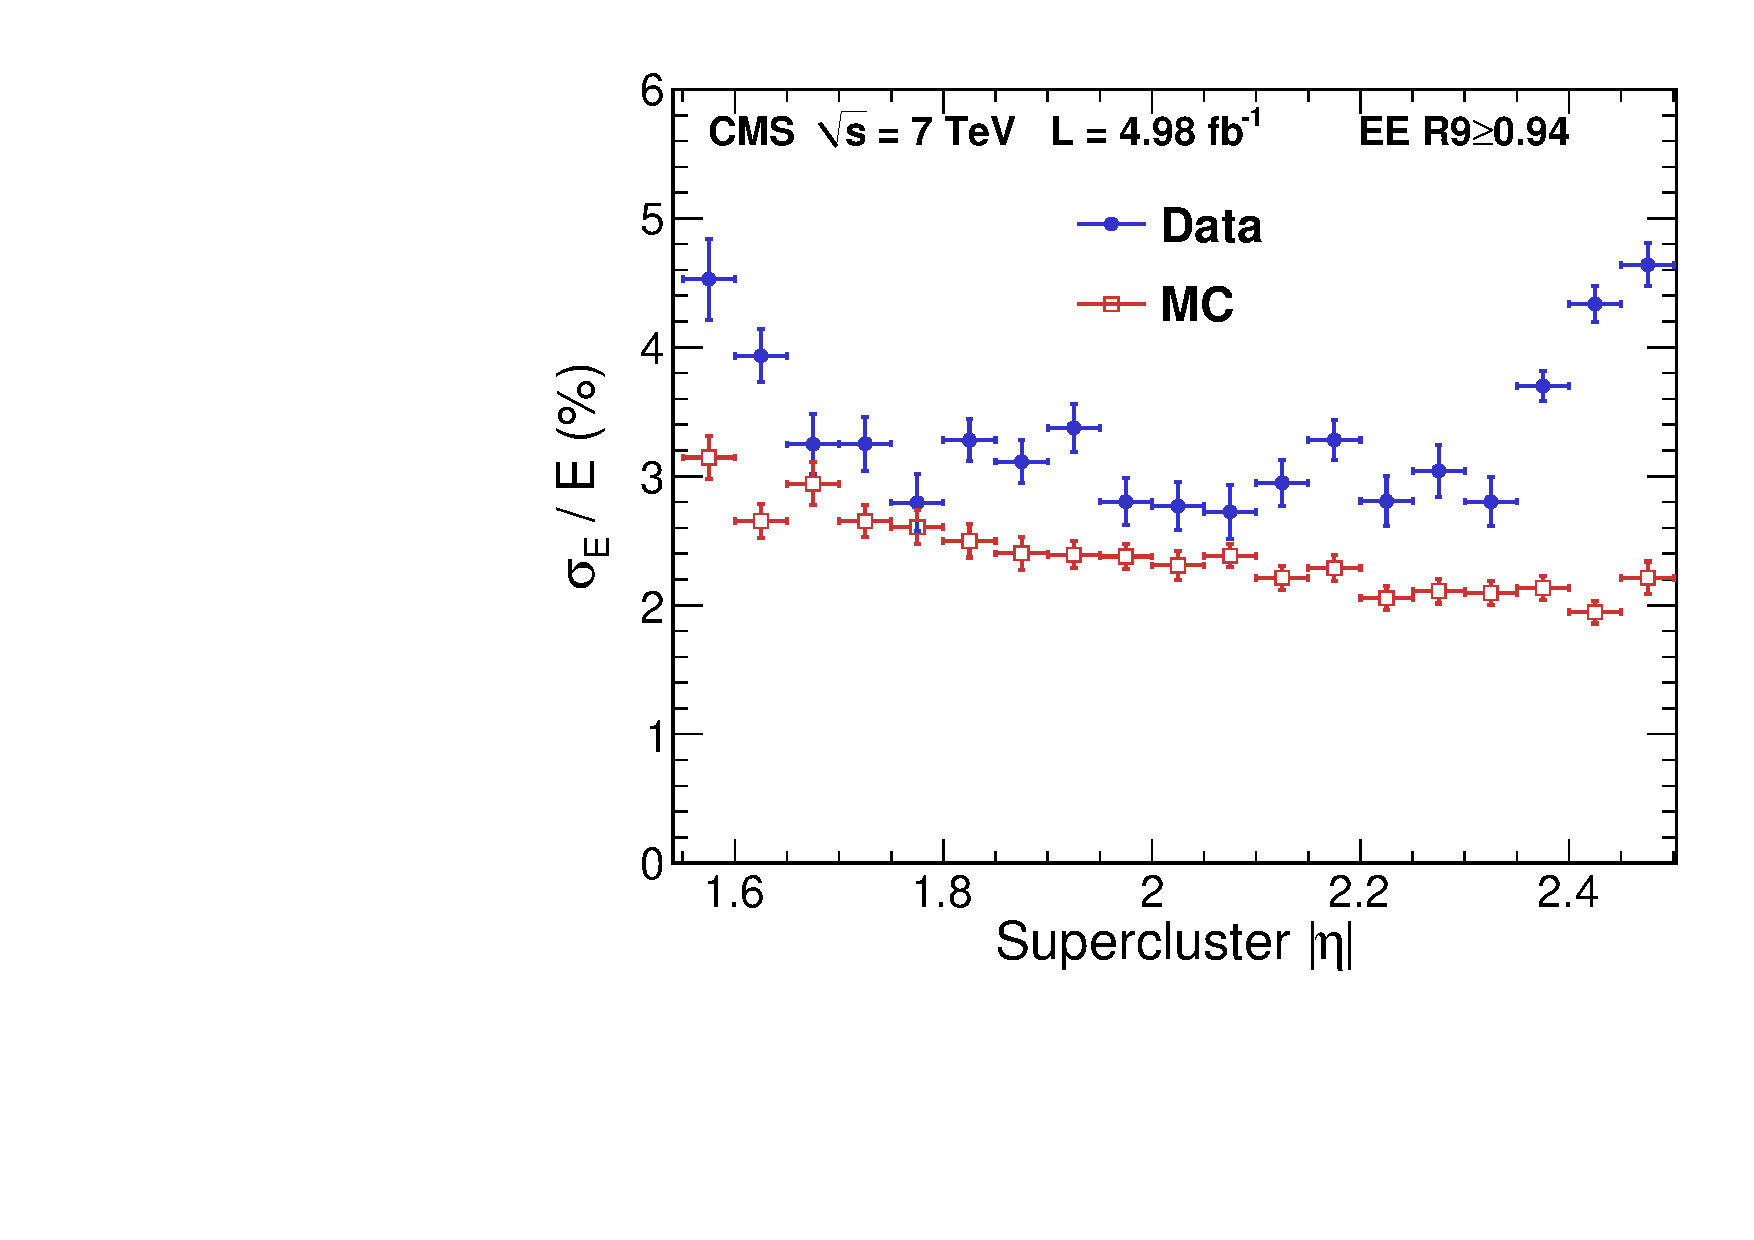
\includegraphics[width=0.39\linewidth]{Experiment/CMS/Image/ECAL/SCe_EtaR9calib_regression_EE_ER_ir9_1.pdf}}
  \subfigure[]
  {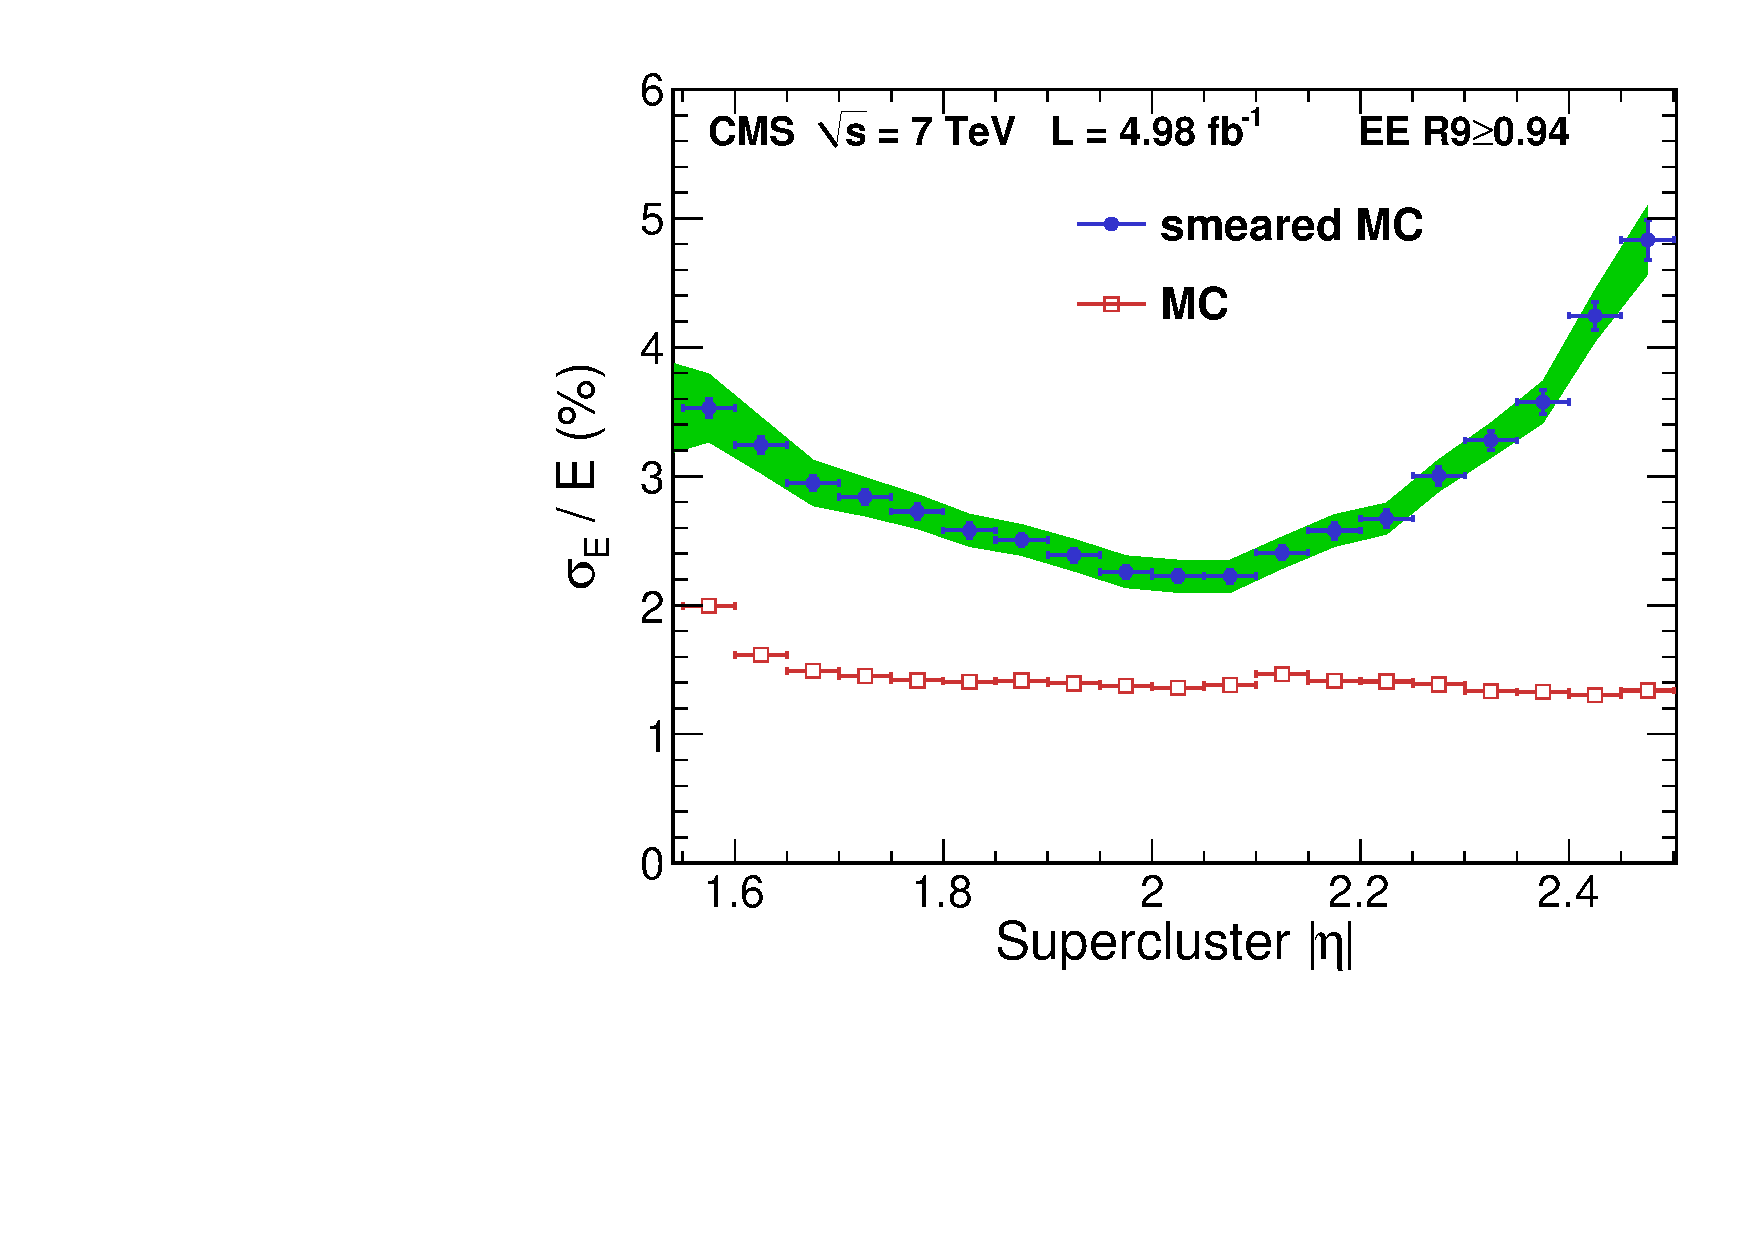
\includegraphics[width=0.39\linewidth]{Experiment/CMS/Image/ECAL/SCphoton_Reso_EE_ER_ir9_1.pdf}}
	\caption{The relative energy resolution of electron and photon as a function
	of supercluster $\eta$ in the barrel and endcap region of the ECAL 
	\cite{Chatrchyan:2013dga}.}
  \label{fig:cms_ecal_reso}
\end{figure}
